% Project report. Build from report/: latexmk -pdf report.tex
% Every result number comes from generated/ (qd_damage.analysis.report); none is typed by hand.
\documentclass[11pt,a4paper]{article}

% ---------------------------------------------------------------- packages
\usepackage[T1]{fontenc}
\usepackage[utf8]{inputenc}
\usepackage{lmodern}
\usepackage[english]{babel}
\usepackage[a4paper,margin=2.5cm]{geometry}
\usepackage{microtype}
\usepackage{amsmath,amssymb}
\usepackage{graphicx}
\usepackage{booktabs}
\usepackage{enumitem}
\usepackage{caption,subcaption}
\usepackage{placeins}
\usepackage[numbers,sort&compress]{natbib}
\usepackage[hidelinks]{hyperref}
\usepackage[capitalise,noabbrev]{cleveref}

% ---------------------------------------------------------------- style
\captionsetup{font=small,labelfont=bf}
\setlist{itemsep=2pt,topsep=4pt}
\renewcommand{\topfraction}{0.9}\renewcommand{\bottomfraction}{0.8}
\renewcommand{\textfraction}{0.07}\renewcommand{\floatpagefraction}{0.75}

% ---------------------------------------------------------------- numbers & figures
% Generated by qd_damage.analysis.report: do not edit.
\newcommand{\BestIntactPct}{18}
\newcommand{\BonusContAbs}{0.14}
\newcommand{\BonusContTrials}{3}
\newcommand{\BonusContWins}{3}
\newcommand{\BonusGridAbs}{0.53}
\newcommand{\BonusGridTrials}{6}
\newcommand{\BonusN}{36}
\newcommand{\BonusNRuns}{3}
\newcommand{\BonusOracleCont}{0.32}
\newcommand{\BonusOracleContBetter}{0}
\newcommand{\BonusOracleGrid}{0.90}
\newcommand{\BonusP}{<0.001}
\newcommand{\CovDCRL}{83.8}
\newcommand{\CovME}{72.3}
\newcommand{\CovPGA}{76.8}
\newcommand{\DiffTopKFive}{+0.02}
\newcommand{\DiffTopKFiveDCRL}{+0.08}
\newcommand{\DiffTopKFiveME}{+0.00}
\newcommand{\DiffTopKFivePGA}{-0.03}
\newcommand{\DiffTopKTen}{+0.01}
\newcommand{\DiffTopKTenDCRL}{+0.04}
\newcommand{\DiffTopKTenME}{+0.01}
\newcommand{\DiffTopKTenPGA}{-0.03}
\newcommand{\DiffTopKThree}{+0.05}
\newcommand{\DiffTopKThreeDCRL}{+0.13}
\newcommand{\DiffTopKThreeME}{+0.01}
\newcommand{\DiffTopKThreePGA}{+0.03}
\newcommand{\ITEAbsDCRL}{0.59}
\newcommand{\ITEAbsFiveDCRL}{0.47}
\newcommand{\ITEAbsFiveME}{0.11}
\newcommand{\ITEAbsFivePGA}{1.47}
\newcommand{\ITEAbsME}{0.11}
\newcommand{\ITEAbsOneDCRL}{0.22}
\newcommand{\ITEAbsOneME}{0.07}
\newcommand{\ITEAbsOnePGA}{1.43}
\newcommand{\ITEAbsPGA}{1.47}
\newcommand{\ITEAbsTenDCRL}{0.59}
\newcommand{\ITEAbsTenME}{0.11}
\newcommand{\ITEAbsTenPGA}{1.47}
\newcommand{\ITEAbsThreeDCRL}{0.47}
\newcommand{\ITEAbsThreeME}{0.10}
\newcommand{\ITEAbsThreePGA}{1.47}
\newcommand{\ITEAbsTwentyDCRL}{0.60}
\newcommand{\ITEAbsTwentyME}{0.12}
\newcommand{\ITEAbsTwentyPGA}{1.47}
\newcommand{\ITEAtFive}{30}
\newcommand{\ITEAtThree}{28}
\newcommand{\ITEAtTwenty}{33}
\newcommand{\ITELosesTopK}{48}
\newcommand{\ITEPctIntact}{33}
\newcommand{\ITEPctIntactDCRL}{33}
\newcommand{\ITEPctIntactME}{24}
\newcommand{\ITEPctIntactPGA}{55}
\newcommand{\ITEPctOracle}{62}
\newcommand{\ITEStopRate}{89}
\newcommand{\ITETiesTopK}{5}
\newcommand{\ITETrials}{5}
\newcommand{\ITETrialsDCRL}{6}
\newcommand{\ITETrialsME}{6}
\newcommand{\ITETrialsPGA}{3}
\newcommand{\ITETrialsQone}{2}
\newcommand{\ITETrialsQthree}{10}
\newcommand{\ITEWinsTopK}{47}
\newcommand{\MaxFitDCRL}{1625}
\newcommand{\MaxFitME}{1235}
\newcommand{\MaxFitPGA}{1922}
\newcommand{\NEvaluations}{512{,}256}
\newcommand{\NIterations}{2000}
\newcommand{\NPairsTopK}{108}
\newcommand{\NScenarios}{12}
\newcommand{\NSeeds}{3}
\newcommand{\NUnits}{36}
\newcommand{\OracleAbsDCRL}{1.14}
\newcommand{\OracleAbsME}{0.23}
\newcommand{\OracleAbsPGA}{1.84}
\newcommand{\OraclePolicies}{731--862}
\newcommand{\PITEAbsMEDCRL}{<0.001}
\newcommand{\PITEAbsMEPGA}{<0.001}
\newcommand{\PITEAbsMin}{<0.001}
\newcommand{\PITEAbsPGADCRL}{=0.002}
\newcommand{\PResMEDCRL}{=0.996}
\newcommand{\PResMEPGA}{=0.532}
\newcommand{\PResMin}{=0.496}
\newcommand{\PResPGADCRL}{=0.496}
\newcommand{\PTopKFive}{=0.445}
\newcommand{\PTopKFiveDCRL}{=0.166}
\newcommand{\PTopKFiveME}{=0.798}
\newcommand{\PTopKFivePGA}{=0.974}
\newcommand{\PTopKTen}{=0.487}
\newcommand{\PTopKTenDCRL}{=0.407}
\newcommand{\PTopKTenME}{=0.451}
\newcommand{\PTopKTenPGA}{=0.944}
\newcommand{\PTopKThree}{=0.009}
\newcommand{\PTopKThreeDCRL}{=0.019}
\newcommand{\PTopKThreeME}{=0.581}
\newcommand{\PTopKThreePGA}{=0.135}
\newcommand{\QDDCRL}{1074k}
\newcommand{\QDME}{814k}
\newcommand{\QDPGA}{962k}
\newcommand{\RLFinetuneEpisodes}{1264}
\newcommand{\RLFinetuneReached}{3/8}
\newcommand{\RLMaxEpisodes}{2000}
\newcommand{\RLScratchEpisodes}{1264}
\newcommand{\RLScratchReached}{3/8}
\newcommand{\RandomAbsFiveDCRL}{0.28}
\newcommand{\RandomAbsFiveME}{0.07}
\newcommand{\RandomAbsFivePGA}{0.47}
\newcommand{\RandomAbsOneDCRL}{0.03}
\newcommand{\RandomAbsOneME}{-0.03}
\newcommand{\RandomAbsOnePGA}{0.10}
\newcommand{\RandomAbsTenDCRL}{0.49}
\newcommand{\RandomAbsTenME}{0.09}
\newcommand{\RandomAbsTenPGA}{0.78}
\newcommand{\RandomAbsThreeDCRL}{0.22}
\newcommand{\RandomAbsThreeME}{0.02}
\newcommand{\RandomAbsThreePGA}{0.21}
\newcommand{\RandomAbsTwentyDCRL}{0.59}
\newcommand{\RandomAbsTwentyME}{0.12}
\newcommand{\RandomAbsTwentyPGA}{1.11}
\newcommand{\RandomAtFive}{16}
\newcommand{\RandomAtThree}{9}
\newcommand{\RandomAtTwenty}{33}
\newcommand{\ResDCRL}{64}
\newcommand{\ResME}{54}
\newcommand{\ResPGA}{73}
\newcommand{\TopKAbsFiveDCRL}{0.37}
\newcommand{\TopKAbsFiveME}{0.10}
\newcommand{\TopKAbsFivePGA}{1.52}
\newcommand{\TopKAbsOneDCRL}{0.22}
\newcommand{\TopKAbsOneME}{0.07}
\newcommand{\TopKAbsOnePGA}{1.43}
\newcommand{\TopKAbsTenDCRL}{0.48}
\newcommand{\TopKAbsTenME}{0.09}
\newcommand{\TopKAbsTenPGA}{1.52}
\newcommand{\TopKAbsThreeDCRL}{0.36}
\newcommand{\TopKAbsThreeME}{0.09}
\newcommand{\TopKAbsThreePGA}{1.47}
\newcommand{\TopKAbsTwentyDCRL}{0.59}
\newcommand{\TopKAbsTwentyME}{0.11}
\newcommand{\TopKAbsTwentyPGA}{1.57}
\newcommand{\TopKAtFive}{30}
\newcommand{\TopKAtThree}{27}
\newcommand{\TopKAtTwenty}{35}

\graphicspath{{../media/final/figures_en/}{../media/final/ite_main/figures_en/}}

\newcommand{\ME}{MAP-Elites}
\newcommand{\PGA}{PGA-ME}
\newcommand{\DCRL}{DCRL-ME}

\begin{document}

% ================================================================ title
\title{Few-Trial Damage Recovery with Quality-Diversity Repertoires\\[4pt]
\large Repertoires built with and without reinforcement learning, adapted with Intelligent Trial \& Error}
\author{Anaïs Azouaoui\\[2pt] \small\url{https://github.com/AnaisAzouaoui/qd-damage-recovery}}
\date{\today}
\maketitle

\begin{abstract}
A legged robot that loses the use of a leg should find a new gait with as few physical trials as possible.
Intelligent Trial \& Error (ITE) does so by searching, with Bayesian optimisation, a repertoire of diverse gaits
learned beforehand in simulation. Recent Quality-Diversity (QD) algorithms build such repertoires with the help of
reinforcement-learning (RL) critics and reach much higher performance, but it is not known whether they keep the
diversity that makes a repertoire useful after damage. On the Brax Ant, we build repertoires at equal budget with
\ME, \PGA{} and \DCRL{} (\NSeeds{} seeds each), measure their resilience to \NScenarios{} damage scenarios, and adapt
them with ITE, simple baselines and RL re-training (TD3), counting episodes on the damaged robot. Repertoires built
with RL are as resilient as those of \ME{} in relative terms and keep much better gaits in absolute terms. ITE needs a
median of \ITETrials{} trials, recovers \ITEPctIntact\% of the progress of the best intact gait (against
\BestIntactPct\% without adaptation), but is barely better than trying gaits in decreasing order of their intact
performance: its small advantage after three trials is gone after five. Except in one case where the intact policy already matched ITE before any training, TD3 needs
more than a thousand episodes to reach the same performance, when it reaches it at all.
\end{abstract}

\begin{figure}[h]
\centering
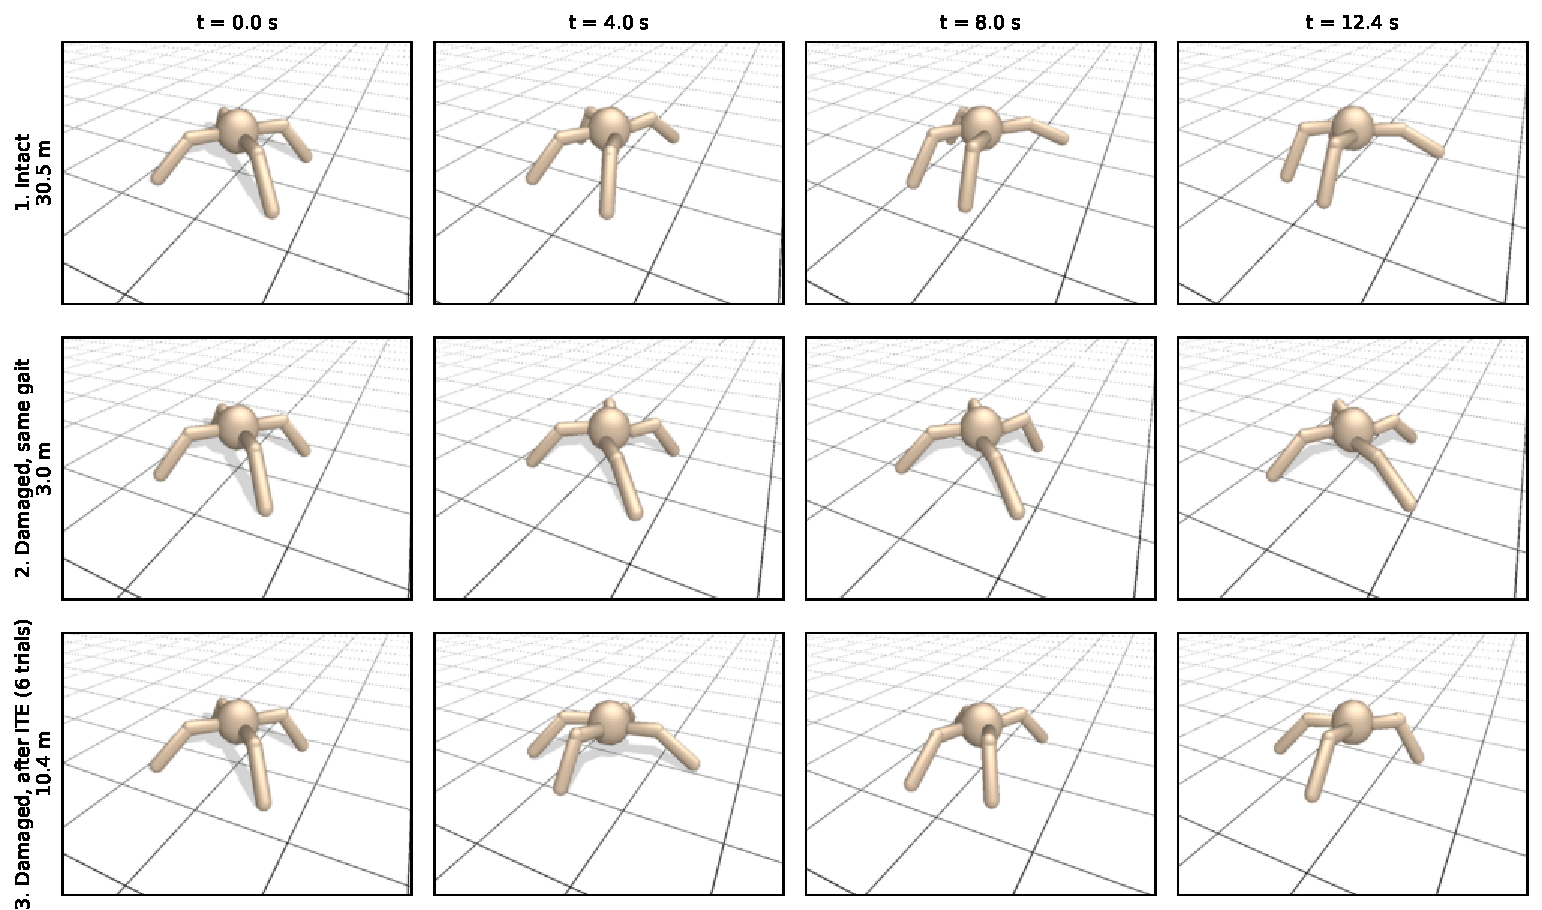
\includegraphics[width=\linewidth]{three_phase_strip}
\caption{The simulated quadruped with its best gait (top), the same gait after the front-right leg is paralysed
(middle), and the gait found by ITE in a few trials (bottom). Distances travelled in 12.5\,s on the left.}
\label{fig:teaser}
\end{figure}

\tableofcontents


% ================================================================ 1
\section{Introduction}
Animals keep walking after an injury because they already know many ways to move: they limp, shift their weight,
use another leg more. \citet{cully2015robots} gave robots the same ability. \emph{Before} any damage, a large
repertoire of diverse gaits is learned in simulation with MAP-Elites \citep{mouret2015illuminating}; \emph{after}
damage, the robot runs Intelligent Trial \& Error (ITE): it tests a promising gait, observes how well it works,
and updates a Gaussian-process model of the performance of \emph{all similar} gaits, so that each trial is
informative about many of them. A damaged hexapod recovered in less than two minutes.

Since then, QD algorithms have been combined with deep RL. PGA-ME \citep{nilsson2021policy} improves half of
the offspring with the gradient of a TD3 critic \citep{fujimoto2018addressing}; DCRL-ME
\citep{faldor2024synergizing} conditions critic and actor on the targeted behaviour descriptor, so that RL can
improve a gait \emph{without changing its style}. These methods produce much better gaits. Whether they also
produce repertoires that are useful after damage is less clear: RL pushes towards high performance, possibly at
the cost of the diversity that adaptation needs. Moreover, adaptation has mostly been evaluated with an
\emph{oracle} that tries every skill on the damaged robot \citep{chalumeau2023neuroevolution}, which says nothing
about the number of trials a real robot would need.

\paragraph{Summary of results} (i) At equal budget, \DCRL{} covers the most cells (\CovDCRL\%) and \PGA{} finds the
fastest gaits (best fitness \MaxFitPGA). The \emph{relative} resilience to damage does not differ significantly between
algorithms, but the best gait left after damage is much better in repertoires built with RL. (ii) ITE stops after a
median of \ITETrials{} trials and recovers \ITEPctIntact\% of the intact progress, against \BestIntactPct\% for the
best intact gait; however, a model-free strategy that tries gaits in decreasing order of intact performance (top-$k$)
does almost as well: ITE is slightly ahead after three trials, mostly on \DCRL{} repertoires, and no longer after five. (iii) RL re-training needs more than a thousand episodes, and
starting from the intact policy does not help. (iv) Searching the continuous descriptor space with the \DCRL{}
conditioned actor, instead of the repertoire cells, is clearly worse.

\paragraph{Questions}
\begin{enumerate}[label=\textbf{Q\arabic*.},leftmargin=2.2em]
  \item At equal budget, are repertoires built with RL (\PGA, \DCRL) more or less \emph{resilient} to damage than
        those of \ME?
  \item How many \emph{trials} does ITE need on each kind of repertoire, compared with simpler strategies?
  \item How does this compare with re-training a policy by RL on the damaged robot, counted in episodes?
\end{enumerate}

% ================================================================ 2
\section{Background and related work}
\subsection{Quality-Diversity and MAP-Elites}
A QD algorithm searches for a \emph{collection} of solutions that are both diverse and high-performing.
MAP-Elites \citep{mouret2015illuminating} discretises a user-defined \emph{behaviour descriptor} space into cells
and keeps, in each cell, the best solution found (its \emph{elite}). At each iteration, elites are selected at
random, mutated, evaluated, and inserted in their cell if they beat its current occupant.

\subsection{QD with reinforcement learning}
Mutations are blind. PGA-ME \citep{nilsson2021policy} trains a TD3 critic on all transitions collected by the
population and uses its gradient to improve half of the offspring. DCG-ME and DCRL-ME \citep{faldor2024synergizing}
condition the critic on a target descriptor, so that the gradient improves a policy while keeping its behaviour,
and also train a descriptor-conditioned actor whose outputs are added to the repertoire.
\citet{chalumeau2023neuroevolution} compared QD methods with skill-discovery RL (DIAYN, DADS, SMERL) on few-shot
adaptation tasks, including a leg dysfunction on Ant: after perturbation, every skill is evaluated and the best
one is kept. QD methods were more robust to large perturbations, and PGA-ME adapted better than MAP-Elites.

\subsection{Damage recovery with repertoires}
ITE \citep{cully2015robots} uses the M-BOA algorithm described in \cref{sec:ite}. Follow-ups removed the need for
resets \citep{chatzilygeroudis2018reset}, selected among several priors \citep{kaushik2020adaptive}, or used
hierarchical repertoires \citep{allard2022online}. We keep the original algorithm and study the effect of
\emph{how the repertoire was built}.

% ================================================================ 3
\section{Experimental setup}
\subsection{Robot, task and behaviour descriptor}
We use the Brax Ant (\texttt{ant\_uni} in QDax \citep{chalumeau2023qdax}): a torso and four legs, each with a hip
and an ankle actuator (8 actions). The reward is the forward velocity plus a survival bonus, minus control and
contact costs, over episodes of 250 steps (12.5\,s). As in the DCRL-ME notebook, rewards are shifted by a constant
and clipped at zero for all algorithms. The descriptor is the fraction of time each foot touches the ground,
$\mathbf{d}\in[0,1]^4$; the repertoire is a centroidal Voronoi tessellation of 1024 cells.

\paragraph{Leg mapping} The mapping from actions to legs was checked in three independent ways (geometry of the
bodies at reset, relative motion of each foot when a single action is applied, and video): actions $(0,1)$,
$(2,3)$, $(4,5)$, $(6,7)$ drive the hip and ankle of the front-left (FL), hind-left (HL), hind-right (HR) and
front-right (FR) legs.

\subsection{Algorithms and budget}
The three algorithms share the environment, the policy architecture (MLP, two hidden layers of 128 units, tanh
output), the repertoire, and the number of evaluations per iteration (256); hyper-parameters specific to each
algorithm are those of the official QDax notebooks (\cref{tab:hparams}). Each run lasts \NIterations{}
iterations, i.e.\ \NEvaluations{} episodes; \NSeeds{} seeds per algorithm. A test checks that the three
configurations only differ by their emitter.

\begin{table}[htbp]
\centering\small
\caption{Main hyper-parameters (full configuration in \texttt{configs/}).}
\label{tab:hparams}
\begin{tabular}{lccc}
\toprule
 & \ME & \PGA & \DCRL \\
\midrule
Offspring per iteration & 256 mutations & 128 mutations + 128 PG & 128 + 64 PG + 64 actor \\
Iso/line variation $\sigma$ & 0.005 / 0.05 & 0.005 / 0.05 & 0.005 / 0.05 \\
Critic & -- & TD3, $256\times256$ & descriptor-cond., $256\times256$ \\
Critic steps / iteration & -- & 300 & 3000 \\
PG steps / iteration & -- & 100 & 150 \\
\bottomrule
\end{tabular}
\end{table}

\subsection{Damage scenarios}
A damage multiplies the actions of some joints by a factor $\lambda$ ($\lambda=0$: paralysed, $\lambda=0.5$:
weakened). Since the torque of an Ant actuator is proportional to its action, this is equivalent to scaling its
strength, as in \citet{chalumeau2023neuroevolution}. We use \NScenarios{} scenarios: each leg paralysed, each leg
weakened, two legs paralysed (FL+HL, same side; FL+FR, both front legs), and one ankle paralysed (FL, HR).

\subsection{Performance scale}\label{sec:scale}
Episodes are noisy (random initial state), and a robot that does not move still collects the survival bonus: its
return $F_0$ was measured at $4.23$ per step (1058.7 per episode). We report
\[ p = \frac{F - F_0}{S}, \qquad S = 1.2 \text{ per step } (300 \text{ per episode}), \]
so that $p\approx0$ for a standing robot and $p\approx1$ for $\approx$15\,m in 12.5\,s, or percentages of the
progress $F-F_0$ of the best intact gait. With this scale, the variance of a single episode's performance is
$\approx10^{-3}$, the value used by \citet{cully2015robots}.

% ================================================================ 4
\section{Methods}
\subsection{Oracle and resilience}
For each repertoire and damage, every policy is evaluated on 4 episodes. The best mean is the \emph{oracle}
performance, an upper bound for any method that picks a gait from the repertoire (it needs 4 episodes for each of the
\OraclePolicies{} policies of a repertoire, for every damage).
The \emph{resilience} of a repertoire to a damage is the fraction of the intact oracle progress still reachable:
$(F^\star_{\text{damaged}}-F_0)/(F^\star_{\text{intact}}-F_0)$.

\subsection{Intelligent Trial \& Error}\label{sec:ite}
Let $P(\mathbf{d}_i)$ be the prior performance of cell $i$ on the intact robot. ITE models the residual between
observed and prior performance with a Gaussian process with a Matérn-5/2 kernel on descriptors:
\begin{align*}
\mu_t(\mathbf{d}) &= P(\mathbf{d}) + \mathbf{k}(\mathbf{d})^\top (K + \sigma_n^2 I)^{-1}\big(\mathbf{y} - P(\mathbf{D}_t)\big),\\
\sigma_t^2(\mathbf{d}) &= \sigma_f^2 - \mathbf{k}(\mathbf{d})^\top (K + \sigma_n^2 I)^{-1}\mathbf{k}(\mathbf{d}),
\end{align*}
where $\mathbf{D}_t$ and $\mathbf{y}$ are the descriptors and observed performances of the gaits tried so far.
The next gait maximises the upper confidence bound $\mu_t + \kappa\sigma_t$; ITE stops when the best observed
performance reaches $\alpha\max_{\mathbf{d}}\mu_t(\mathbf{d})$. One trial is \emph{one} episode on the damaged robot.

\paragraph{Prior} The fitness stored in a repertoire comes from a single noisy episode, and MAP-Elites keeps the
luckiest evaluations: elites are over-estimated (on development repertoires, the correlation between stored and
re-evaluated fitness is 0.88, and the ``best'' cell of a \ME{} repertoire performs worse than a standing robot once
re-evaluated). As the repertoire is built offline in simulation, we re-evaluate it on the intact robot (4 episodes)
and use this as prior; the best-intact baseline uses the same values.

\paragraph{Hyper-parameters} With the values of \citet{cully2015robots} (length-scale 0.4, unit signal variance,
noise $10^{-3}$), ITE stopped after very few trials and plateaued. The residuals have a variance of 0.03--0.06, not 1,
and a large nugget (neighbouring cells differ). We therefore fitted $(\ell,\sigma_f^2,\sigma_n^2)$ by maximising the
marginal likelihood on \emph{development} repertoires (short runs of the three algorithms, never used for the results):
$\ell=0.4$, $\sigma_f^2=0.05$, $\sigma_n^2=0.02$ (log-likelihood $+4059$ against $-1280$ for the original values).
$\kappa=0.05$ and $\alpha=0.9$ are those of \citet{cully2015robots}; values of $\kappa$ from 0.05 to 2 made little
difference on the development set.

\subsection{Baselines}
\emph{Best-intact}: replay the best intact gait (no adaptation, one trial). \emph{Top-$k$}: try cells by decreasing
prior, without a model. \emph{Random}: try cells at random. All methods run for 20 trials and are repeated 5 times
per (repertoire, damage); the quality of the recommended gait (best observed so far) is measured with its oracle mean.

\subsection{Statistics}
The repetitions of an adaptation only differ by episode noise, so they are averaged first: the statistical unit is a
(repertoire, damage) pair, i.e.\ \NUnits{} units per algorithm. Algorithms are compared with two-sided Mann-Whitney
tests on these units, and two adaptation methods with paired two-sided Wilcoxon signed-rank tests. Units of the same
seed share a repertoire and are not fully independent, so p-values should be read as indicative. Medians in the tables
are taken over all repetitions.

\subsection{RL re-training}
TD3 (QDax implementation) is trained on the damaged robot, either from scratch or starting from the best intact
\DCRL{} policy (same architecture; the critic starts from scratch), on 4 damages (FR leg paralysed, HL leg weakened,
FL+FR legs paralysed, FL ankle paralysed) and 2 seeds, for \RLMaxEpisodes{} episodes with 16 robots in parallel and
one gradient step per transition. The deterministic policy is evaluated on 8 episodes after every 16 training
episodes. In the reported runs the starting policy is the elite with the highest \emph{stored} fitness, because the
oracle ran in parallel; for seed~1 it is also the best re-evaluated elite, for seed~0 it is a different elite whose
re-evaluated intact fitness is 1.4\% below the best one. The code now starts from the best re-evaluated elite.

% ================================================================ 5
\section{Results}
\subsection{Repertoires on the intact robot}
\begin{figure}[htbp]
\centering
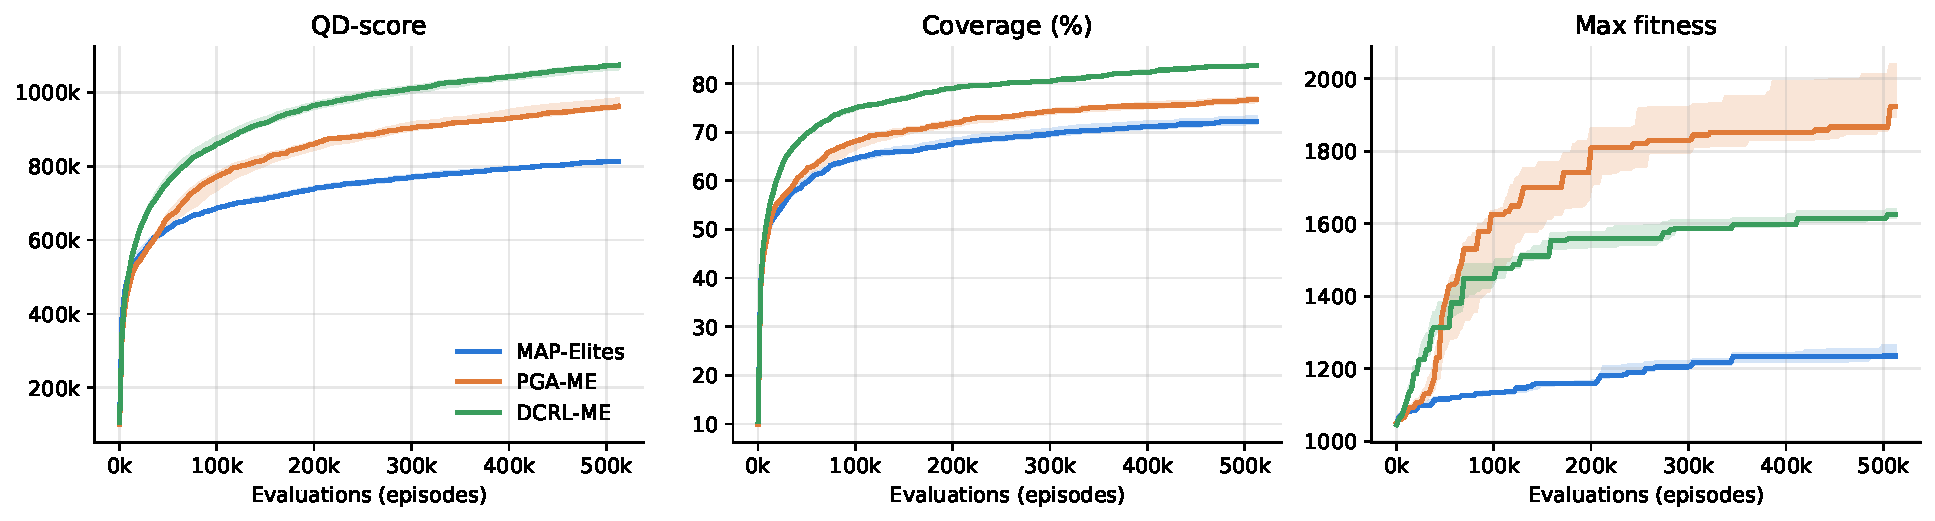
\includegraphics[width=\linewidth]{repertoire_progress}
\caption{QD-score, coverage and best fitness during training (median and inter-quartile range over \NSeeds{} seeds).}
\label{fig:progress}
\end{figure}

\begin{table}[htbp]
\centering\small
\caption{Repertoires at the end of training (median over seeds).}
\label{tab:quality}
\begin{tabular}{lrrr}
\toprule
Algorithm & Coverage (\%) & Max fitness & QD-score ($\times 10^3$) \\
\midrule
MAP-Elites & 72.3 & 1235 & 814 \\
PGA-ME & 76.8 & 1922 & 962 \\
DCRL-ME & 83.8 & 1625 & 1074 \\
\bottomrule
\end{tabular}

\end{table}

Both RL-based algorithms improve over \ME{} at equal budget (\cref{fig:progress,tab:quality}), in different ways.
\DCRL{} fills the most cells and reaches the highest QD-score, which is consistent with its descriptor-conditioned
critic improving gaits \emph{without changing their style}. \PGA{} finds by far the fastest gaits (median best fitness
\MaxFitPGA{} against \MaxFitDCRL{} for \DCRL{} and \MaxFitME{} for \ME): its unconditioned critic pushes offspring towards
high reward, wherever they land in the grid. The fastest gait we inspected (\PGA) is a bounding gait in which the feet
touch the ground only briefly. The stored fitness of these elites is optimistic (\cref{sec:discussion}).

\FloatBarrier
\subsection{Resilience to damage (Q1)}
\begin{figure}[htbp]
\centering
\begin{subfigure}{0.40\linewidth}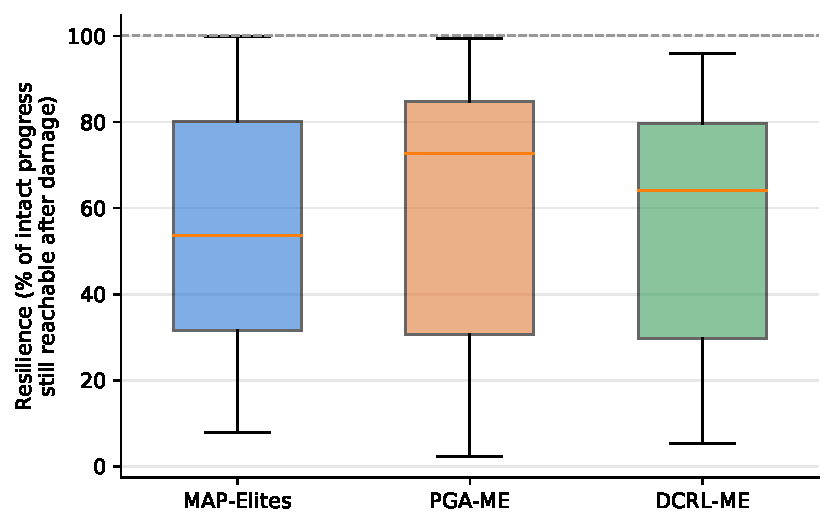
\includegraphics[width=\linewidth]{resilience_by_algo}\caption{All damages}\end{subfigure}\hfill
\begin{subfigure}{0.58\linewidth}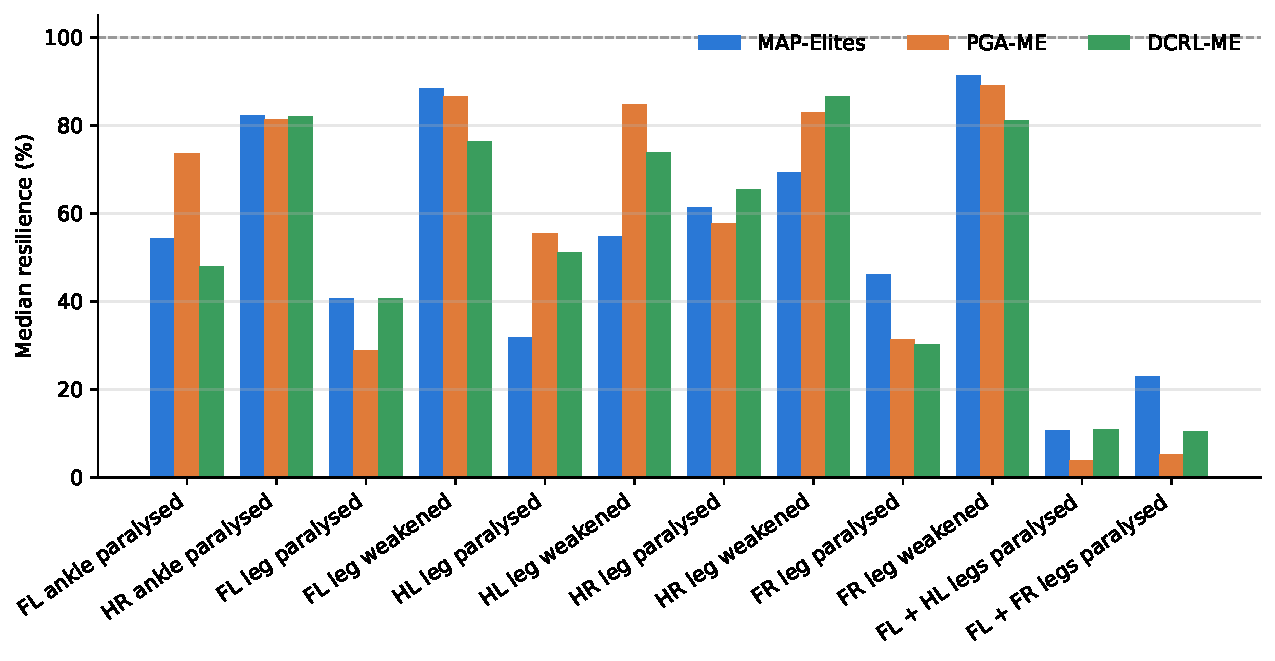
\includegraphics[width=\linewidth]{resilience_by_damage}\caption{By damage (median over seeds)}\end{subfigure}
\caption{Resilience: share of the intact oracle progress still reachable after damage.}
\label{fig:resilience}
\end{figure}

\begin{table}[htbp]
\centering\small
\caption{Resilience (\%) and absolute oracle performance $p$ after damage (median over seeds).}
\label{tab:resilience}
\resizebox{\linewidth}{!}{\begin{tabular}{lrrrrrr}
\toprule
Damage & MAP-Elites (\%) & PGA-ME (\%) & DCRL-ME (\%) & MAP-Elites ($v$) & PGA-ME ($v$) & DCRL-ME ($v$) \\
\midrule
FL ankle paralysed & 54 & 74 & 48 & 0.28 & 1.86 & 0.83 \\
HR ankle paralysed & 82 & 81 & 82 & 0.35 & 2.06 & 1.48 \\
FL leg paralysed & 41 & 29 & 41 & 0.21 & 0.73 & 0.73 \\
FL leg weakened & 88 & 87 & 76 & 0.38 & 2.20 & 1.32 \\
HL leg paralysed & 32 & 55 & 51 & 0.13 & 1.72 & 0.92 \\
HL leg weakened & 55 & 85 & 74 & 0.24 & 2.33 & 1.32 \\
HR leg paralysed & 61 & 58 & 65 & 0.23 & 1.79 & 1.18 \\
HR leg weakened & 69 & 83 & 87 & 0.28 & 2.15 & 1.56 \\
FR leg paralysed & 46 & 31 & 30 & 0.20 & 0.97 & 0.54 \\
FR leg weakened & 91 & 89 & 81 & 0.40 & 2.25 & 1.42 \\
FL + HL legs paralysed & 11 & 4 & 11 & 0.06 & 0.10 & 0.19 \\
FL + FR legs paralysed & 23 & 5 & 10 & 0.12 & 0.16 & 0.18 \\
\bottomrule
\end{tabular}
}
\end{table}

In relative terms, the three kinds of repertoires are equally resilient: the median share of the intact progress
that remains reachable after damage is \ResME\% for \ME, \ResPGA\% for \PGA{} and \ResDCRL\% for \DCRL, and none of
the pairwise differences is significant (Mann-Whitney, $p\PResMEPGA$, $p\PResMEDCRL$ and $p\PResPGADCRL$;
\cref{fig:resilience}). We therefore find no sign that RL makes repertoires less useful after damage. In absolute terms,
the difference is large (\cref{tab:resilience}): after damage, the best gait available is worth a median
$p=\OracleAbsPGA$ in \PGA{} repertoires, $p=\OracleAbsDCRL$ in \DCRL{} ones and only $p=\OracleAbsME$ in \ME{} ones.
Weakening a leg is usually mild; paralysing a whole leg removes roughly half of the progress; with two paralysed
legs, no repertoire keeps a useful gait.

\FloatBarrier
\subsection{Adaptation in a few trials (Q2)}
\begin{figure}[htbp]
\centering
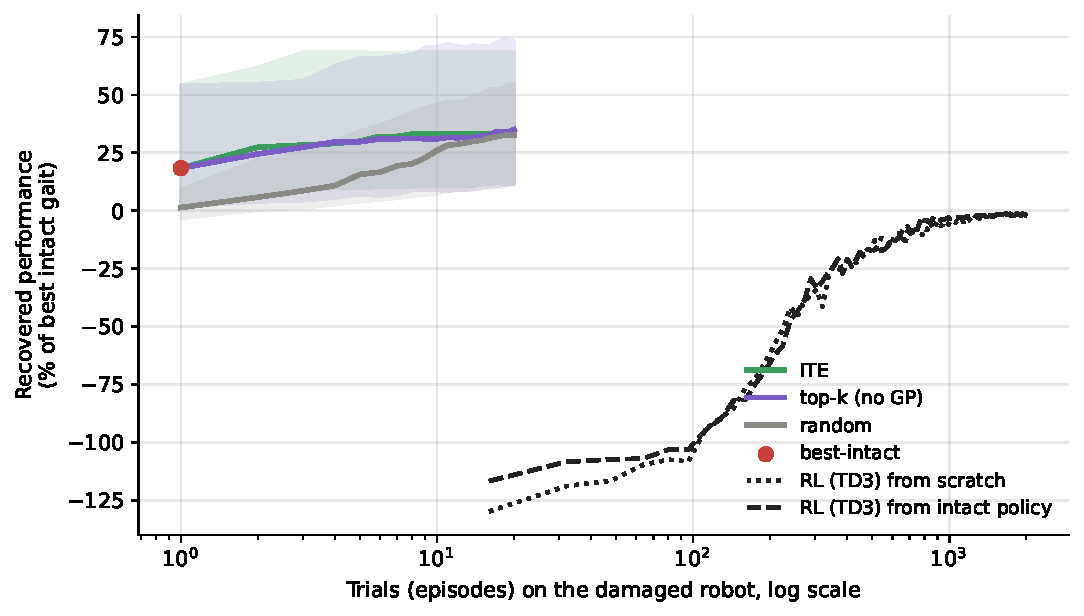
\includegraphics[width=0.78\linewidth]{performance_vs_trials}
\caption{Performance of the recommended gait against the number of trials on the damaged robot (median and IQR over
repertoires, damages and repetitions; each repertoire relative to its own best intact gait). RL curves are relative
to the best intact \DCRL{} gait.}
\label{fig:trials}
\end{figure}

\begin{table}[htbp]
\centering\small
\caption{Adaptation methods (median over repertoires, damages and repetitions). ``\% intact'': share of the progress
of the best intact gait; ``\% oracle'': share of the best gait available after damage.}
\label{tab:methods}
\begin{tabular}{lrrrr}
\toprule
Method & Trials & \% intact & \% oracle & Absolute $v$ \\
\midrule
ITE & 5 & 33 & 62 & 0.37 \\
top-$k$ (no GP) & 20 & 35 & 77 & 0.40 \\
random & 20 & 33 & 60 & 0.31 \\
best-intact & 1 & 18 & 34 & 0.19 \\
\bottomrule
\end{tabular}

\vspace{1em}
\caption{Share of the intact progress (\%) recovered after a given number of trials (median).}
\label{tab:equal}
\begin{tabular}{lrrrrr}
\toprule
Method & 1 trial & 3 trials & 5 trials & 10 trials & 20 trials \\
\midrule
ITE & 18 & 28 & 30 & 33 & 33 \\
top-$k$ (no GP) & 18 & 27 & 30 & 31 & 35 \\
random & 1 & 9 & 16 & 26 & 33 \\
\bottomrule
\end{tabular}

\end{table}

ITE meets its stopping criterion in \ITEStopRate\% of the runs, after a median of \ITETrials{} trials (IQR
\ITETrialsQone--\ITETrialsQthree). The recommended gait recovers \ITEPctIntact\% of the progress of the best intact
gait, against \BestIntactPct\% when the best intact gait is simply replayed, and \ITEPctOracle\% of what an exhaustive
search of the repertoire would find (\cref{tab:methods}). Random search is much slower (\RandomAtThree\% after three
trials, against \ITEAtThree\% for ITE).

The comparison with top-$k$, which tries gaits in decreasing order of intact performance without any model, is less
favourable: after three trials ITE reaches \ITEAtThree\% and top-$k$ \TopKAtThree\%; after 20 trials, \ITEAtTwenty\%
and \TopKAtTwenty\% (\cref{fig:trials,tab:equal}). Paired over the \NPairsTopK{} (repertoire, damage) units, ITE is
better than top-$k$ after five trials in \ITEWinsTopK\% of them, equal in \ITETiesTopK\% and worse in \ITELosesTopK\%
(Wilcoxon $p\PTopKFive$). After three trials ITE has a small advantage (mean difference \DiffTopKThree{} in $p$,
$p\PTopKThree$), which comes mostly from \DCRL{} repertoires (\DiffTopKThreeDCRL, $p\PTopKThreeDCRL$) and disappears
after five and ten trials (\cref{tab:itevstopk}). The pooled medians of \cref{tab:equalalgo} suggest a larger gap on
\DCRL{} repertoires ($\ITEAbsTenDCRL$ against $\TopKAbsTenDCRL$ after ten trials), but the paired test does not support it
($p\PTopKTenDCRL$): unit by unit, ITE is better as often as it is worse (\cref{tab:itevstopk}). On \PGA{} repertoires, the best intact gait already keeps most of its
performance ($p=\ITEAbsOnePGA$ at the first trial). On \ME{} repertoires, all methods stay close to a standing robot.

\begin{table}[htbp]
\centering\small
\caption{ITE against top-$k$ at equal numbers of trials: mean difference in absolute performance $p$ (ITE $-$ top-$k$),
number of units where ITE is better / equal / worse, and paired Wilcoxon test, over the (repertoire, damage) units.}
\label{tab:itevstopk}
\resizebox{\linewidth}{!}{\begin{tabular}{lrrr}
\toprule
Repertoire & 3 trials & 5 trials & 10 trials \\
\midrule
MAP-Elites & $+0.01$ (18/0/18; $p=0.581$) & $+0.00$ (16/0/20; $p=0.798$) & $+0.01$ (20/0/16; $p=0.451$) \\
PGA-ME & $+0.03$ (19/4/13; $p=0.135$) & $-0.03$ (18/1/17; $p=0.974$) & $-0.03$ (18/0/18; $p=0.944$) \\
DCRL-ME & $+0.13$ (20/1/15; $p=0.019$) & $+0.08$ (17/4/15; $p=0.166$) & $+0.04$ (17/2/17; $p=0.407$) \\
\bottomrule
\end{tabular}
}
\end{table}

\begin{table}[htbp]
\centering\small
\caption{Absolute performance $p$ of the recommended gait at equal numbers of trials, by repertoire (median).}
\label{tab:equalalgo}
\begin{tabular}{lrrrrr}
\toprule
Repertoire -- method & 1 trial & 3 trials & 5 trials & 10 trials & 20 trials \\
\midrule
MAP-Elites -- ITE & 0.07 & 0.10 & 0.11 & 0.11 & 0.12 \\
MAP-Elites -- top-$k$ & 0.07 & 0.09 & 0.10 & 0.09 & 0.11 \\
MAP-Elites -- random & -0.03 & 0.02 & 0.07 & 0.09 & 0.12 \\
PGA-ME -- ITE & 1.43 & 1.47 & 1.47 & 1.47 & 1.47 \\
PGA-ME -- top-$k$ & 1.43 & 1.47 & 1.52 & 1.52 & 1.57 \\
PGA-ME -- random & 0.10 & 0.21 & 0.47 & 0.78 & 1.11 \\
DCRL-ME -- ITE & 0.22 & 0.47 & 0.47 & 0.59 & 0.60 \\
DCRL-ME -- top-$k$ & 0.22 & 0.36 & 0.37 & 0.48 & 0.59 \\
DCRL-ME -- random & 0.03 & 0.22 & 0.28 & 0.49 & 0.59 \\
\bottomrule
\end{tabular}

\end{table}

\begin{table}[htbp]
\centering\small
\caption{ITE on each kind of repertoire (median over seeds, damages and repetitions).}
\label{tab:itealgo}
\begin{tabular}{lrrr}
\toprule
Repertoire & Trials & \% intact & Absolute $v$ \\
\midrule
MAP-Elites & 6 & 24 & 0.11 \\
PGA-ME & 3 & 55 & 1.47 \\
DCRL-ME & 6 & 33 & 0.59 \\
\bottomrule
\end{tabular}

\end{table}

What a robot finally gets depends mostly on how its repertoire was built (\cref{tab:itealgo}): with ITE, the
recommended gait is worth $p=\ITEAbsPGA$ with \PGA, $p=\ITEAbsDCRL$ with \DCRL{} and $p=\ITEAbsME$ with \ME{}
(Mann-Whitney on the (repertoire, damage) units: $p\PITEAbsMEPGA$ for \ME{} against \PGA, $p\PITEAbsMEDCRL$ against
\DCRL{} and $p\PITEAbsPGADCRL$ between \PGA{} and \DCRL; at the level of seeds, every \PGA{} repertoire is above every
\DCRL{} repertoire, itself above every \ME{} repertoire). \Cref{fig:itetrials,fig:map} show one ITE run.

\begin{figure}[htbp]
\centering
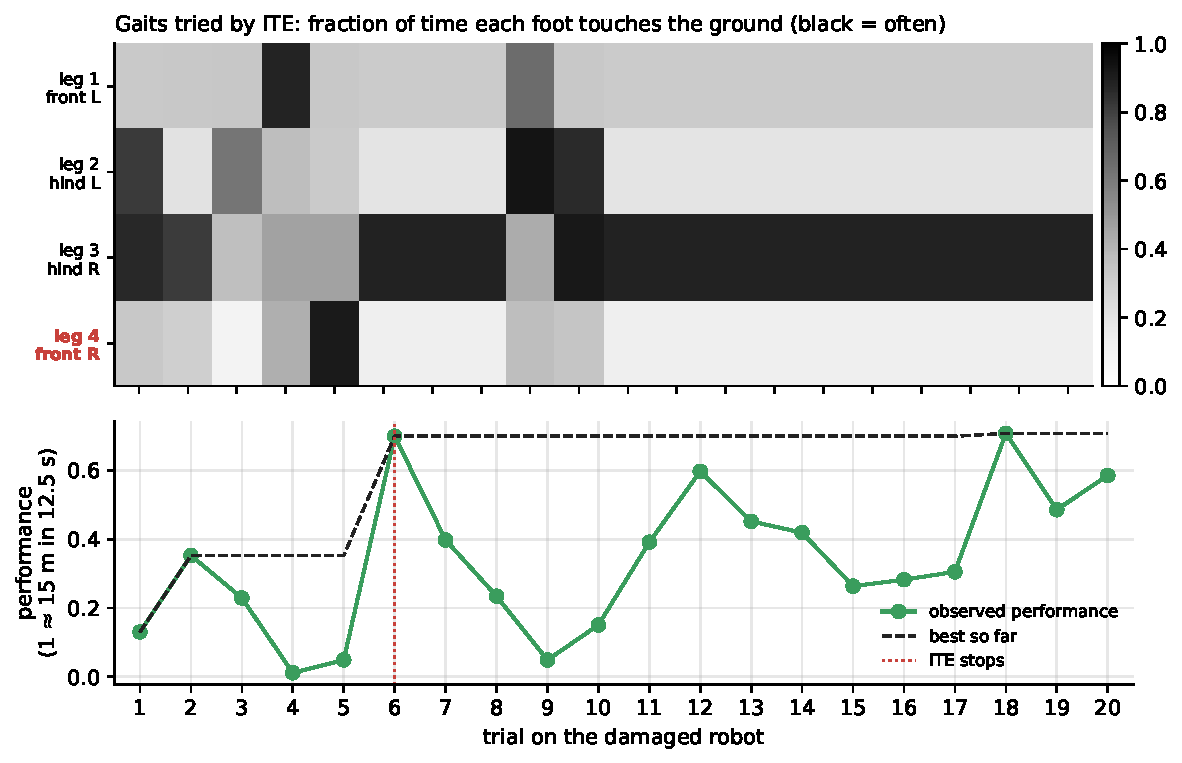
\includegraphics[width=0.85\linewidth]{ite_trials}
\caption{One ITE run on a \DCRL{} repertoire (front-right leg paralysed; the five repetitions all recommend the same
gait, after 6 or 7 trials, and this one used 6): feet-contact profile of each gait tried, and its observed performance.}
\label{fig:itetrials}
\end{figure}

\begin{figure}[htbp]
\centering
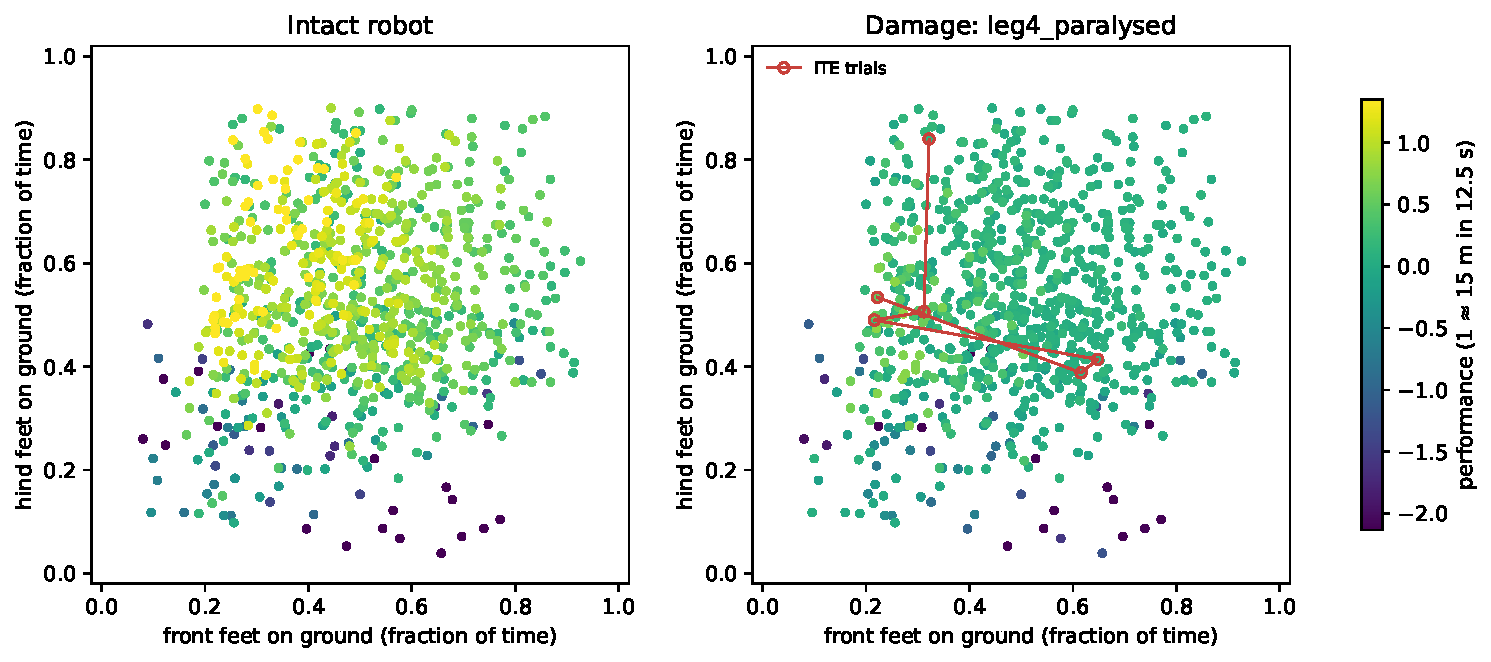
\includegraphics[width=0.95\linewidth]{map_before_after}
\caption{The same repertoire before and after damage (front vs hind feet contact), and the gaits tried by ITE.}
\label{fig:map}
\end{figure}

\FloatBarrier
\subsection{Comparison with RL re-training (Q3)}
\begin{figure}[htbp]
\centering
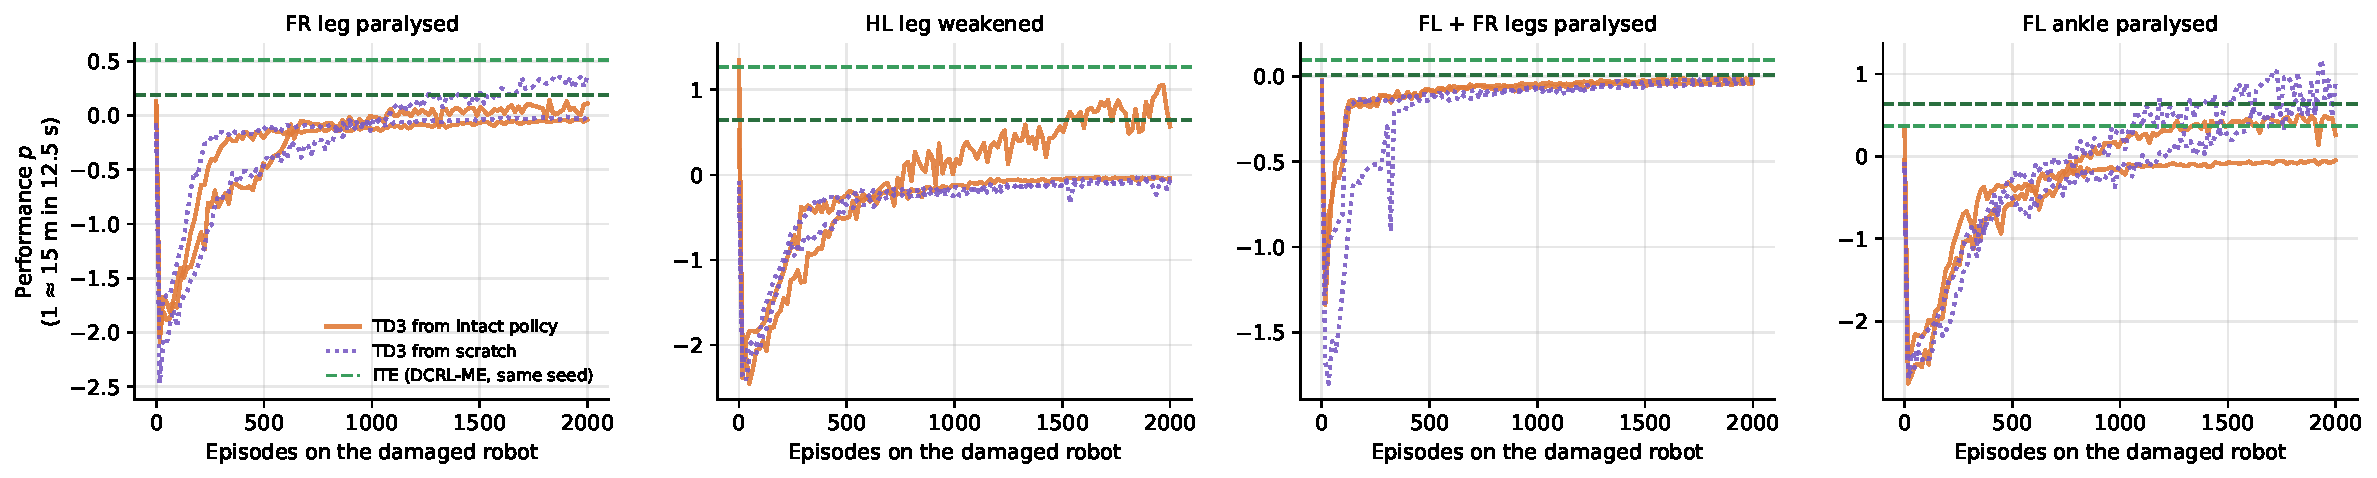
\includegraphics[width=\linewidth]{rl_curves}
\caption{TD3 on the damaged robot, from scratch and from the best intact \DCRL{} policy (two seeds each), against the
performance of the gait found by ITE on the \DCRL{} repertoire of the same seed (dashed lines).}
\label{fig:rl}
\end{figure}

\IfFileExists{generated/table_rl.tex}{%
\begin{table}[htbp]
\centering\small
\caption{Episodes needed by TD3 to match the gait found by ITE (\DCRL{} repertoire of the same seed); ``--'': not
reached within \RLMaxEpisodes{} episodes.}
\label{tab:rl}
\begin{tabular}{lrrrrr}
\toprule
Damage & ITE trials & Scratch & Fine-tune & Warm-up & Pre-trained critic \\
\midrule
FL ankle paralysed, seed 0 & 10.0 & 1072 & -- & 496 & 112 \\
FL ankle paralysed, seed 1 & 5.6 & 1808 & -- & 400 & 576 \\
HL leg weakened, seed 0 & 1.4 & -- & 0 & 0 & 1088 \\
HL leg weakened, seed 1 & 6.4 & -- & 1536 & 336 & 224 \\
FR leg paralysed, seed 0 & 6.6 & -- & -- & 496 & 192 \\
FR leg paralysed, seed 1 & 15.0 & 1264 & -- & 224 & 192 \\
FL + FR legs paralysed, seed 0 & 18.8 & -- & -- & 1008 & 1344 \\
FL + FR legs paralysed, seed 1 & 20.0 & -- & -- & 720 & 720 \\
\bottomrule
\end{tabular}

\end{table}}{}

Within \RLMaxEpisodes{} episodes, TD3 from scratch matches the gait found by ITE in \RLScratchReached{} runs (median
\RLScratchEpisodes{} episodes when it does), and TD3 from the intact policy in \RLFinetuneReached{} runs
(\cref{fig:rl,tab:rl}), against 1 to 20 trials for ITE. In one of the latter cases, the intact policy already matched
ITE before any training. Otherwise, starting from the intact policy does not help: its performance collapses at the first
evaluation (after 16 episodes), and the robot has to learn again almost from scratch. The most likely cause is that the
policy starts following the gradient of a new critic that has not been trained yet; we did not test it. A pre-trained
critic, a warm-up period without policy updates, or a smaller policy learning rate could make fine-tuning useful.

\FloatBarrier
\subsection{Bonus: searching the continuous descriptor space}
\begin{figure}[htbp]
\centering
\begin{minipage}{0.48\linewidth}\centering
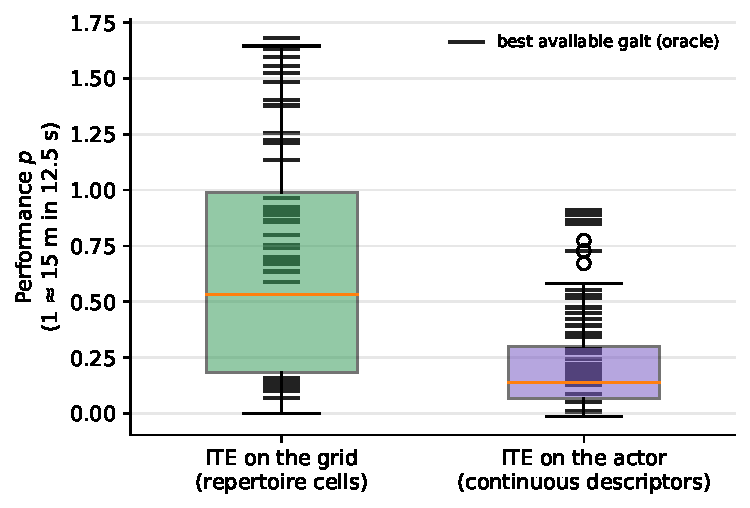
\includegraphics[width=\linewidth]{bonus_grid_vs_continuous}
\end{minipage}\hfill
\begin{minipage}{0.48\linewidth}\centering\small
\begin{tabular}{lrrr}
\toprule
ITE search space & Trials & Found $p$ & Oracle $p$ \\
\midrule
Grid (repertoire cells) & 6 & 0.53 & 0.90 \\
Continuous (conditioned actor) & 3 & 0.14 & 0.32 \\
\bottomrule
\end{tabular}

\end{minipage}
\caption{ITE on the cells of a \DCRL{} repertoire against ITE on 2048 gaits generated by its descriptor-conditioned
actor for targets spread over $[0,1]^4$ (\BonusNRuns{} dedicated runs, same runs for both).}
\label{fig:bonus}
\end{figure}

\DCRL{} also learns an actor $\pi(a\mid o,\mathbf{d})$ that should produce a gait with any requested feet-contact
profile $\mathbf{d}$. We let ITE search 2048 such gaits instead of the repertoire cells, on \BonusNRuns{} dedicated
\DCRL{} runs where the actor was saved. The answer is clearly negative (\cref{fig:bonus}): the gaits produced by the actor
are much weaker than the elites (best available gait after damage $p=\BonusOracleCont$ against $p=\BonusOracleGrid$, and
never better in any of the (run, damage) pairs), and ITE on the actor finds $p=\BonusContAbs$ against $p=\BonusGridAbs$
on the grid (better in only \BonusContWins{} of the \BonusN{} (run, damage) pairs; Wilcoxon $p\BonusP$). The actor is a
useful source of offspring during training, but it does not replace the elites that were selected and refined.

% ================================================================ 6
\FloatBarrier
\section{Discussion}\label{sec:discussion}
\paragraph{Why ITE is not much better than top-$k$} ITE helps when trying one gait tells something about
\emph{similar} gaits. Here, the effect of damage is only weakly correlated between neighbouring cells of the
feet-contact descriptor: on development repertoires, a large part of the variance of the residuals is already present
between the closest cells (the ``nugget'' of the variogram, from a few percent of the variance for \ME{} to more than half
for \PGA), and the noise variance fitted by maximum likelihood (0.02) is not small compared with the signal variance
(0.05). The Gaussian process can therefore generalise little, while the
re-evaluated intact performance is already a good guide. A descriptor closer to what a damage affects (e.g.\ the torque
or contact pattern of each leg separately) might make the model more useful.

\paragraph{Noisy elites} A repertoire stores the fitness of a single noisy episode, and MAP-Elites keeps the luckiest
ones: elites are over-estimated. Re-evaluating the repertoire before damage, offline in simulation, is cheap and was
necessary for both ITE and the best-intact baseline. This is the problem studied by uncertain QD.

\paragraph{The oracle is optimistic} The oracle is the maximum of noisy means over $\sim$1000 cells, so it is biased
upwards; percentages of the oracle under-estimate all methods.

\paragraph{Counting episodes, not compute} In simulation, RL consumes thousands of episodes in minutes; on a real robot,
each episode costs time, wear and supervision. We therefore compare trials and episodes, not wall-clock time.

\section{Limitations}
Simulation only; one robot; damages modelled as action scaling; one repertoire size and one budget; \NSeeds{} seeds per
algorithm, so the (repertoire, damage) units used in the tests are not independent and the p-values are indicative;
ITE hyper-parameters fitted on development repertoires of the same algorithms; RL re-training with standard TD3 settings
only (no tuning of the fine-tuning variant), 2 seeds and 4 damages.

\section{Conclusion and future work}
Repertoires built with the help of RL critics are not less useful after damage: they are as resilient in relative
terms and keep much better gaits in absolute terms, so that the quality of the repertoire, more than the adaptation
algorithm, decides how well a damaged robot walks. ITE finds a good gait in a handful of trials, orders of magnitude
fewer than RL re-training, but in this setting most of its benefit comes from a good prior: a simple ranking of
re-evaluated gaits is almost as good. Future work: descriptors that make the effect of damage smoother, pre-trained
critics for RL fine-tuning, and tests on a physical robot.

\small
\bibliographystyle{plainnat}
\bibliography{refs}

\normalsize
\appendix
\section{Reproducibility}
\begin{small}\ttfamily\noindent
python -m qd\_damage.repertoires --algo \{me,pgame,dcrlme\} --seed S\\
python -m qd\_damage.oracle --runs results/repertoires/<run>\\
python -m qd\_damage.adaptation --runs results/repertoires/<run>\\
python -m qd\_damage.rl\_retrain --scenario <s> --variant \{scratch,finetune\} --seed S\\
python -m qd\_damage.analysis.report
\end{small}
Versions: QDax 0.5.0, JAX 0.4.28, Brax 0.10.4 (pinned; see \texttt{requirements-lock.txt}). Repertoires were built
on Kaggle (2$\times$ Tesla T4). Every run stores its configuration, seed, code commit, library versions and device.

\end{document}
